\documentclass[12pt,a4paper]{article}
\usepackage[utf8]{inputenc}
\usepackage[T1]{fontenc}
\usepackage[portuguese]{babel}
\usepackage{amsmath}
\usepackage{amsfonts}
\usepackage{amssymb}
\usepackage{geometry}
\usepackage{hyperref}
\geometry{a4paper, margin=2.5cm}
\usepackage{graphicx}
\usepackage{float}

\title{Trabalho Prático 2 \\ Modelagem de Redes Sociais Acadêmicas}
\author{Thales Alves Amaral \\ \small{Departamento de Ciência da Computação} \\ \small{Universidade Federal de Minas Gerais (UFMG)} \\ \small{Belo Horizonte - MG - Brasil}}
\date{}

\begin{document}
\maketitle

\section{Introdução}

Este documento descreve a implementação do sistema ConectaDCC, uma rede social acadêmica que mantém usuários, seus temas de interesse e relações de seguimento entre usuários. O programa processa comandos de cadastro, atualização e consulta, e produz, para cada linha de entrada, uma saída no formato especificado pelo enunciado.

Resumidamente, o problema consiste em dois grafos. O primeiro é o grafo social, direcionado e não ponderado, em que uma aresta $u \rightarrow v$ indica que o usuário $u$ segue o usuário $v$. O segundo é o grafo de temas, não direcionado, não ponderado e bipartido, em que uma aresta conecta um usuário a um tema de seu interesse.

A solução utiliza TADs para representar usuários, temas, nós, dicionário, grafo e ordenação. O TAD Grafo foi implementado de forma genérica, permitindo representar tanto o grafo social quanto o grafo de temas, mesmo ambos possuindo características diferentes. Na parte obrigatória, ele suporta duas representações internas: lista de adjacência e matriz de adjacência, e permite migrar de uma forma a outra durante a execução sem perda de dados e relações. As saídas que exigem ordem crescente de identificador são ordenadas por uma implementação de Mergesort estável. Como pontos extras, também foram implementados o comando \texttt{P}, que recomenda usuários a partir de uma combinação entre proximidade social e afinidade temática, e uma representação por matriz esparsa, voltada a reduzir o uso de memória em grafos com poucas arestas.

\section{Método}

O projeto foi implementado em C++11, usando programação orientada a objetos (POO) e
tipos abstratos de dados (TADs). A estrutura é modular, separada em headers e arquivos
de implementação. Os módulos são:

\begin{itemize}
    \item \textbf{Usuário} - TAD que armazena as informações básicas de um usuário:
    identificador, nome e idade.

    \item \textbf{Tema} - TAD que representa um tema cadastrado no sistema. Cada tema
    possui identificador, nome e tipo, que pode ser acadêmico (A) ou pessoal (P).

    \item \textbf{Nó} - Estrutura usada como conteúdo associado a cada vértice do grafo.
    Cada nó armazena um identificador externo e um tipo, indicando se o vértice representa
    um usuário ou um tema. Essa separação é necessária porque o usuário de identificador
    0 e o tema de identificador 0 são entidades diferentes, apesar de terem o mesmo valor
    numérico como identificador externo.

    \item \textbf{Dicionário} - TAD que liga os identificadores usados na
    entrada aos objetos armazenados no programa e aos vértices internos dos grafos. Como
    os identificadores de usuários e temas são sequenciais e começam em 0, o dicionário foi
    implementado com arrays indexados diretamente pelo identificador. Ele armazena os
    usuários, os temas e os índices correspondentes no grafo social e no grafo de temas.

    \begin{itemize}
        \item \textbf{Separação entre identificador externo e índice interno} - O
        identificador externo é o valor usado nos comandos de entrada e nas saídas. O
        índice interno é a posição do vértice dentro do array de vértices do TAD Grafo. O
        grafo opera apenas com índices internos, e o dicionário faz a conversão quando
        necessário. Essa separação é especialmente importante no grafo de temas, pois
        usuários e temas possuem sequências independentes de identificadores, ou seja, um tema e um usuário podem compartilhar o mesmo identificador externo, mas não podem ser armazenados no mesmo espaço do array.
    \end{itemize}

    \item \textbf{Grafo} - TAD central da implementação. Ele foi desenvolvido para
    representar tanto o grafo social quanto o grafo de temas. O grafo social é direcionado,
    pois a relação de seguimento não é necessariamente mútua. Já o grafo de temas é não
    direcionado e bipartido, pois representa associações entre usuários e temas.

    \begin{itemize}
        \item \textbf{Lista de adjacência} - Na representação por lista, cada vértice
        possui uma lista encadeada com seus vizinhos de saída, isto é, os vértices
        alcançados por arestas que saem dele. Para grafos direcionados, também é mantida
        uma lista de entrada, que permite obter os seguidores de um usuário sem percorrer
        todas as listas do grafo social. As arestas são inseridas no início da lista, já que a
        ordenação das saídas que precisam estar ordenadas é feita posteriormente, deixando
        a inserção mais simples.

        \item \textbf{Matriz de adjacência} - Na representação por matriz, o grafo usa
        uma matriz booleana em que a posição $[i][j]$ indica se existe uma aresta do
        vértice $i$ para o vértice $j$, onde $i$ e $j$ representam os índices internos dos
        vértices. Essa representação facilita a verificação de existência de aresta, mas exige
        mais memória, principalmente quando o grafo possui muitos vértices e poucas
        arestas (grafo esparso).

        \item \textbf{Migração entre representações} - O comando \texttt{A} realiza a
        troca entre lista e matriz. Na migração de lista para matriz, uma nova matriz é
        alocada e as arestas das listas são copiadas para ela. Na migração de matriz para
        lista, a matriz é percorrida e as listas encadeadas são construídas a partir dela. Depois da
        migração, a representação antiga é liberada. Assim, o estado do grafo é
        preservado, mas apenas uma representação fica ativa por vez, o que evita desperdício
        de memória.
    \end{itemize}

    \item \textbf{Ordenação} - Módulo auxiliar usado para ordenar identificadores externos
    antes da impressão das consultas. A ordenação usa um Mergesort estável implementado manualmente.
    Essa ordenação é usada nas consultas \texttt{LT}, \texttt{LC}, \texttt{LS} e \texttt{LA},
    que exigem saída em ordem crescente de identificador.

    \item \textbf{BuffersConsulta} - Para evitar alocações repetidas durante as
        consultas, foram usados buffers auxiliares reutilizáveis. Esses buffers armazenam
        temporariamente os índices internos retornados pelo grafo e, em seguida, os
        identificadores externos que serão ordenados e impressos. Assim, o programa evita
        criar e destruir arrays a cada consulta. Foi criado para modularizar o código e acrescentar o
        comando \texttt{P} do ponto extra em um módulo único, o que deixa o projeto mais organizado.

    \item \textbf{Main} - Faz a leitura da entrada, o processamento sequencial
    dos comandos e impressão das saídas. A função principal mantém o dicionário, o grafo
    social, o grafo de temas, o módulo de ordenação e os buffers auxiliares usados nas
    consultas.

    \begin{itemize}
        \item \textbf{Cadastros} - Nos comandos \texttt{T} e
        \texttt{U}, o programa cria os objetos correspondentes, adiciona os vértices nos
        grafos e registra os mapeamentos no dicionário. Quando um tema é cadastrado, ele é
        inserido apenas no grafo de temas. Quando um usuário é cadastrado, ele é inserido
        nos dois grafos: no grafo social, para participar das relações de seguimento, e no
        grafo de temas, para ser ligado aos seus temas de interesse.

        \item \textbf{Atualizações} - Nos comandos \texttt{S} e
        \texttt{R}, o dicionário converte os identificadores externos dos usuários em
        índices internos do grafo social. Depois disso, a aresta correspondente é inserida ou
        removida no TAD Grafo.

        \item \textbf{Consultas} - A consulta \texttt{LT} obtém os
        vizinhos do usuário no grafo de temas e filtra apenas os vértices que representam
        temas. A consulta \texttt{LC} obtém os predecessores do usuário no grafo social.
        A consulta \texttt{LS} obtém os vizinhos de saída no grafo social. A consulta
        \texttt{LA} percorre os usuários seguidos por um usuário e mantém apenas aqueles
        que também possuem uma aresta no sentido contrário. A consulta \texttt{Q}
        verifica as duas possíveis arestas entre dois usuários. A consulta \texttt{G}
        testa a existência da aresta entre um usuário e um tema no grafo de temas. Por
        fim, a consulta \texttt{F} conta quantos usuários estão ligados a um tema.
    \end{itemize}
\end{itemize}

\subsection{Pontos extras}

\subsubsection{Matriz esparsa}

A matriz esparsa foi adicionada como um terceiro modo de armazenamento do grafo,
acionado pelo modo \texttt{E}. Diferente da matriz booleana, ela não aloca todas as
combinações possíveis entre vértices. Ela guarda apenas os pares de índices internos
que representam arestas existentes, usando um array para as linhas e outro para as
colunas.

No grafo não direcionado, uma associação é guardada nos dois sentidos, como acontece
na lista de adjacência. A interface pública do TAD Grafo foi mantida, então o restante
do programa continua usando as mesmas operações de inserção, remoção, consulta e
listagem. A diferença fica apenas na forma interna de armazenar as arestas.

Essa representação foi pensada para economizar memória em grafos esparsos. Em troca,
ela não oferece o mesmo acesso direto da matriz completa a uma posição $[i][j]$. Por
isso, algumas operações precisam procurar a aresta entre os pares armazenados. A
migração também foi estendida para aceitar esse modo, preservando as arestas entre uma
representação e outra.

\subsubsection{Comando \texttt{P}}

No comando \texttt{P}, o módulo \texttt{Recomendador} concentra a lógica da
consulta de recomendação de usuários. O comando recebe um
usuário base, um valor \texttt{topk} e dois pesos: um para proximidade social e outro
para afinidade temática. A implementação reutiliza o grafo social, o grafo de temas e
o dicionário já existentes, sem alterá-los, mantendo a mesma separação entre identificadores externos
e índices internos dos grafos.

Primeiro, o identificador do usuário da entrada é convertido para o índice interno do grafo
social. A partir desse vértice, é executada uma busca em largura (BFS) no grafo social para
calcular a menor distância do usuário base até os demais usuários. As
distâncias são armazenadas em um buffer auxiliar, e usuários não alcançáveis permanecem
com distância \texttt{-1}.

Em seguida, os temas do usuário base são marcados uma única vez em um array auxiliar.
Para cada candidato, o programa percorre seus temas no grafo de temas e calcula a afinidade temática pela razão entre a quantidade de temas compartilhados
e a quantidade total de temas distintos dos dois usuários. O próprio
usuário base e os usuários que ele já segue diretamente não são considerados
candidatos válidos.

Para cada candidato válido, a pontuação é calculada por:

\[
score = peso\_prox \cdot proximidade + peso\_afin \cdot afinidade
\]
Sendo os pesos os valores definidos pela entrada.

A proximidade social é dada por $2/d$, quando existe uma distância social válida $d$,
e por zero caso contrário. Candidatos com pontuação zero continuam sendo válidos, pois
a consulta recomenda os melhores candidatos disponíveis até o limite definido por
\texttt{topk}.

As recomendações são guardadas em um buffer com o identificador do usuário e sua
pontuação. Depois, esse buffer é ordenado por um Mergesort auxiliar, diferente do encontrado em \texttt{Ordenacao}, já que \texttt{score} tem tipo \texttt{double}: primeiro pela maior pontuação
e, em caso de empate, pelo menor identificador. Na comparação entre pontuações, foi
usada uma pequena tolerância numérica (\texttt{epsilon}) para lidar com valores calculados em
\texttt{double}. Ao final, o programa imprime o usuário consultado e os usuários recomendados, até \texttt{topk}.

\subsection{Compilação e execução}

O projeto utiliza um Makefile para automatizar a compilação. Para compilar:

\begin{verbatim}
make all
\end{verbatim}

O executável gerado é \texttt{bin/tp2.out}. Para executar o programa:

\begin{verbatim}
./bin/tp2.out < input.txt
\end{verbatim}

Para limpar os arquivos compilados:

\begin{verbatim}
make clean
\end{verbatim}

\section{Análise de Complexidade}

\subsection{Variáveis utilizadas}

As variáveis usadas na análise são:

\begin{itemize}
    \item $n$: número de usuários cadastrados;
    \item $m$: número de temas cadastrados;
    \item $V_s = n$: número de vértices do grafo social;
    \item $V_t = n + m$: número de vértices do grafo de temas;
    \item $E_s$: número de arestas do grafo social;
    \item $E_t$: número de arestas do grafo de temas;
    \item $r$: quantidade de temas informados no cadastro de um usuário;
\item $d_t(u)$: grau do usuário $u$ no grafo de temas;
    \item $k$: quantidade de elementos retornados por uma consulta de listagem;
    \item $d^+(u)$: grau de saída de um vértice $u$;
    \item $d^-(u)$: grau de entrada de um vértice $u$;
    \item $c$: número de candidatos válidos encontrados pela consulta \texttt{P};
\end{itemize}

Como o sistema pode usar lista ou matriz de adjacência, algumas operações possuem custos
diferentes dependendo da representação ativa.

\subsection{Complexidade de espaço}

Os TADs Usuário e Tema armazenam apenas os dados básicos das entidades e ocupam
espaço $O(1)$ por objeto. O TAD Dicionário mantém arrays de usuários, temas e
mapeamentos entre identificadores externos e índices internos dos grafos. Como esses
arrays são indexados diretamente pelos IDs, o espaço usado por eles é $O(n + m)$.

\subsubsection{Lista de adjacência}

Na representação por lista de adjacência, o espaço depende da quantidade de vértices e
arestas armazenadas. O grafo social possui $n$ vértices e $E_s$ arestas. Além da lista de
saída, também é mantida uma lista de entrada para facilitar consultas de seguidores. Isso
duplica a quantidade de células associadas às arestas sociais, mas não altera a ordem
assintótica. Portanto, o espaço do grafo social em lista é $O(n + E_s)$.

O grafo de temas possui $n + m$ vértices e $E_t$ arestas entre usuários e temas.
Como ele é não direcionado, cada aresta é armazenada nas duas direções na lista de
adjacência, mas esse fator constante também não altera a ordem assintótica. Assim, o
espaço do grafo de temas em lista é $O(n + m + E_t)$.

Somando a complexidade dos dois grafos, o espaço total da lista de adjacência é:

\[
O(n + m + E_s + E_t)
\]

\subsubsection{Matriz de adjacência}

Na representação por matriz de adjacência, o espaço depende do quadrado do número de
vértices. O grafo social usa uma matriz $n \times n$, enquanto o grafo de temas usa uma
matriz $(n+m) \times (n+m)$. Assim, o espaço total em matriz é
$O(n^2 + (n+m)^2)$. Como $(n+m)^2$ domina $n^2$ assintoticamente, a complexidade
pode ser resumida a:

\[
O((n+m)^2)
\]

Além disso, o programa usa buffers auxiliares nas consultas para armazenar índices internos,
identificadores externos e o vetor auxiliar do Mergesort. Esses buffers têm tamanho
proporcional ao maior grafo, naturalmente o grafo de temas, logo ocupam $O(n+m)$ espaço
adicional.

\subsection{Complexidade de tempo}

O Dicionário usa arrays indexados diretamente pelos identificadores. Por isso, recuperar
usuários, temas ou índices internos dos grafos custa $O(1)$.

\subsubsection{Grafo}

As operações básicas do TAD Grafo têm os seguintes custos:

\begin{center}
\begin{tabular}{|c|c|c|}
\hline
\textbf{Operação} & \textbf{Lista de adjacência} & \textbf{Matriz de adjacência} \\
\hline
Inserir aresta & $O(1)$ & $O(1)$ \\
\hline
Remover aresta & $O(d^+(u) + d^-(v))$ & $O(1)$ \\
\hline
Verificar aresta & $O(d^+(u))$ & $O(1)$ \\
\hline
Listar vizinhos & $O(d^+(u))$ & $O(V)$ \\
\hline
Listar predecessores & $O(d^-(u))$ & $O(V)$ \\
\hline
\end{tabular}
\end{center}

Na lista, verificar uma aresta pode exigir percorrer a lista encadeada do vértice
de origem. Já a remoção, no grafo direcionado, pode exigir percorrer tanto a lista de
saída da origem quanto a lista de entrada do destino. No pior caso, esses graus podem ser
proporcionais ao número de vértices do grafo. Na matriz, essas operações são diretas,
pois basta acessar uma posição da matriz.

A adição de vértices custa $O(1)$ enquanto há capacidade disponível nos arrays internos.
Quando ocorre redimensionamento, o custo depende da representação ativa: em lista, os
arrays de vértices e ponteiros são realocados e copiados, com custo $O(V)$; em matriz, é
necessário criar uma matriz maior e copiar a região antiga, com custo $O(V^2)$.

O comando \texttt{A}, que realiza a migração entre lista e matriz, é uma das operações
mais caras. Na migração de lista para matriz, é necessário inicializar a nova matriz e copiar
as arestas existentes. O custo é:

\[
O(V^2 + E)
\]

Na migração de matriz para lista, é necessário percorrer toda a matriz para reconstruir as
listas de adjacência. O custo é:

\[
O(V^2)
\]

Nessas expressões, $V$ e $E$ se referem ao grafo que está sendo migrado. Como o comando
\texttt{A} migra tanto o grafo social quanto o grafo de temas, o custo total é dominado
pelo maior deles, no caso, pelo grafo de temas.

\subsubsection{Cadastros e atualizações}

Os comandos de cadastro têm custo simples. O comando \texttt{T} cadastra
um tema e adiciona um vértice ao grafo de temas, com custo $O(1)$ sem redimensionamento.
O comando \texttt{U} cadastra um usuário, adiciona um vértice no grafo social, adiciona
um vértice no grafo de temas e cria as arestas para os temas informados. Se o usuário
possui $r$ temas de interesse, o custo é $O(r)$ sem redimensionamento. Quando há
redimensionamento, o custo dos cadastros é dominado pelo custo de realocação da
representação ativa.

Os comandos \texttt{S} e \texttt{R} atualizam o grafo social. A inserção de seguimento
(\texttt{S}) custa $O(1)$ nas duas representações. A remoção (\texttt{R}) custa $O(d^+(u) + d^-(v))$ em lista, pois a aresta precisa ser
removida da lista de saída da origem e da lista de entrada do destino, e $O(1)$ em matriz.

\subsubsection{Consultas}

As consultas \texttt{LT}, \texttt{LC}, \texttt{LS} e \texttt{LA} precisam imprimir elementos
em ordem crescente de identificador. Para isso, os identificadores externos coletados são
ordenados com Mergesort estável. Se a consulta retorna $k$ elementos, a ordenação custa
$O(k \log k)$.

\textbf{\texttt{LT} -} lista os temas de um usuário. Em lista, o custo para obter os vizinhos
do usuário no grafo de temas é proporcional ao seu grau. Chamando esse grau de
$d_t(u)$, o custo é $O(d_t(u) + k \log k)$. Em matriz, é necessário varrer a linha
correspondente ao usuário no grafo de temas, com custo $O(V_t + k \log k)$.

\textbf{\texttt{LC} -} lista seguidores. Em lista, ela usa a lista de entrada do grafo social,
com custo $O(d^-(u) + k \log k)$. Em matriz, precisa varrer a coluna do usuário, com
custo $O(n + k \log k)$.

\textbf{\texttt{LS} -} lista os usuários seguidos. Em lista, ela usa a lista de saída do
usuário, com custo $O(d^+(u) + k \log k)$. Em matriz, precisa varrer a linha do usuário,
com custo $O(n + k \log k)$.

\textbf{\texttt{LA} -} lista amigos, isto é, usuários que possuem relação mútua com o
usuário consultado. Em lista, o programa percorre os seguidos de $u$ e, para cada seguido
$v$, testa se existe a aresta $v \rightarrow u$. Como cada teste em lista pode custar
$O(d^+(v))$, o pior caso é $O(n^2 + k \log k)$. Em matriz, cada teste de reciprocidade é
$O(1)$, então o custo é $O(n + k \log k)$.

\textbf{\texttt{Q} -} verifica as duas possíveis arestas entre dois usuários. Em lista, o
custo é $O(d^+(u) + d^+(v))$, pois são feitas duas verificações de aresta. Em matriz, o
custo é $O(1)$.

\textbf{\texttt{G} -} verifica se existe uma aresta entre um usuário e um tema no grafo de
temas. Em lista, o custo é proporcional ao grau do usuário no grafo de temas, no pior caso
$O(V_t)$. Em matriz, o custo é $O(1)$.

\textbf{\texttt{F} -} calcula a popularidade de um tema. Em lista, basta percorrer os
vizinhos do tema no grafo de temas, com custo proporcional ao número de usuários ligados
a ele, no pior caso $O(n)$. Em matriz, é necessário varrer a linha do tema no grafo de temas,
com custo $O(V_t)$.

Em suma, a lista de adjacência usa menos memória e tende a ser melhor quando
os grafos são esparsos. A matriz de adjacência gasta mais memória, mas tende a ser melhor
nas operações que apenas verificam se uma aresta existe.

\subsection{Pontos extras}

\subsubsection{Matriz esparsa}

Na matriz esparsa, o espaço deixa de depender de todas as posições possíveis da matriz.
O grafo guarda apenas os pares de vértices que possuem aresta, além do vetor de vértices.
Assim, o espaço fica em $O(V + E)$. Considerando os dois grafos do projeto, isso resulta
em $O(n + m + E_s + E_t)$.

O custo de inserir uma aresta é $O(1)$, pois o par é colocado no fim dos
arrays. Já remover, verificar aresta, listar vizinhos e listar predecessores podem exigir
percorrer os pares guardados, então custam $O(E)$ no pior caso. Na prática, essa
representação economiza memória, mas pode perder tempo quando muitas operações
precisam procurar arestas.

A migração entre lista e matriz esparsa percorre as arestas existentes, com custo
$O(V + E)$. Quando a troca envolve a matriz completa, o custo pode voltar a depender de
$V^2$, pois a matriz booleana precisa ser percorrida.

\subsubsection{Comando \texttt{P}}

A consulta \texttt{P} recomenda usuários combinando proximidade social e afinidade
temática. Para isso, ela é dividida em três etapas principais.

Primeiro, é executada uma
busca em largura no grafo social a partir do usuário base, calculando as menores
distâncias direcionadas até os demais usuários. Essa etapa custa $O(n + E_s)$ na
representação por lista de adjacência e $O(n^2)$ na representação por matriz, pois nesse
caso a obtenção dos vizinhos exige varrer linhas da matriz.

Depois, o programa percorre os usuários cadastrados, descarta candidatos inválidos e
calcula a afinidade temática dos candidatos válidos pela razão entre a quantidade de temas
em comum e a quantidade total de temas distintos dos dois usuários, usando os temas
armazenados no grafo de temas. No pior caso, essa etapa custa $O(n^2 + E_t)$ em lista,
considerando as verificações de seguimento direto e a varredura das relações de interesse,
e $O(n \cdot V_t)$ em matriz, pois os temas de cada candidato podem exigir a varredura
de uma linha do grafo de temas.

Por fim, se $c$ candidatos válidos forem encontrados, eles são ordenados por Mergesort
de acordo com o score calculado, com custo $O(c \log c)$. 

O espaço auxiliar total da
consulta é $O(n + m)$, referente aos buffers de distâncias, fila da busca, marcação de
temas e vetor de recomendações.

\section{Estratégias de Robustez}

O enunciado define que toda entrada é válida, portanto não foi necessário
implementar um sistema complexo de tratamento de erros. Ainda assim, algumas decisões
foram adotadas para reduzir riscos de inconsistência e falhas de memória.

\begin{itemize}
    \item \textbf{Separação entre IDs e índices internos -} o programa nunca usa diretamente
    os identificadores da entrada como posições nos grafos. O TAD Dicionário centraliza
    os mapeamentos entre IDs externos e índices internos, evitando confusão entre usuários
    e temas com o mesmo identificador numérico.

    \item \textbf{Inicialização das estruturas -} matrizes booleanas são inicializadas com
    \texttt{false}, e os arrays de mapeamento do Dicionário são inicializados com
    \texttt{-1}. Isso evita leituras de valores não inicializados.

    \item \textbf{Buffers reutilizáveis -} as consultas usam buffers auxiliares reaproveitados
    para armazenar índices internos e identificadores externos. Isso reduz alocações
    repetidas durante a execução e deixa mais clara a posse da memória.

    \item \textbf{Preservação na migração -} a troca entre lista e matriz foi implementada
    copiando todas as arestas da representação ativa antes de liberar a antiga. Assim, a
    mudança de armazenamento não altera o estado lógico dos grafos.
    
\end{itemize}

\section{Análise Experimental}

O objetivo central da análise experimental foi comparar o comportamento das duas
representações obrigatórias do TAD Grafo: lista de adjacência e matriz de adjacência. Para isso,
foram geradas entradas sintéticas variando o número de usuários, a densidade do grafo
social, a quantidade de temas, o número médio de temas por usuário e o perfil das
operações executadas. A densidade social foi definida como a razão entre o número
de arestas existentes no grafo social e o número máximo de arestas possíveis entre os
usuários. Os pontos extras foram avaliados separadamente, para não misturar seus
resultados com a comparação principal.

As medições foram feitas em execuções controladas da implementação, usando entradas
equivalentes para as representações comparadas. Em cada cenário principal, foi alterada
apenas a representação inicial do grafo, entre lista e matriz. Na análise da matriz esparsa,
também foi incluído o modo \texttt{E}. Cada configuração foi executada 5 vezes, e o
valor reportado corresponde à mediana dessas execuções.

Foram avaliados o tempo médio por operação e uma estimativa de memória estrutural
dos grafos. Essa estimativa considera os principais componentes das representações,
como vértices, ponteiros, células de lista, matriz booleana e arrays da matriz esparsa,
não correspondendo necessariamente ao consumo total do processo no sistema operacional.

\subsection{Impacto do número de usuários}

A Figura~\ref{fig:escala-memoria} mostra o impacto do crescimento do número de usuários. Nesse
experimento, o número de usuários varia de 100 a 1500, mantendo fixos a densidade social
e o perfil de carga. O número de temas foi definido proporcionalmente ao número de
usuários.

\begin{figure}[H]
    \centering
    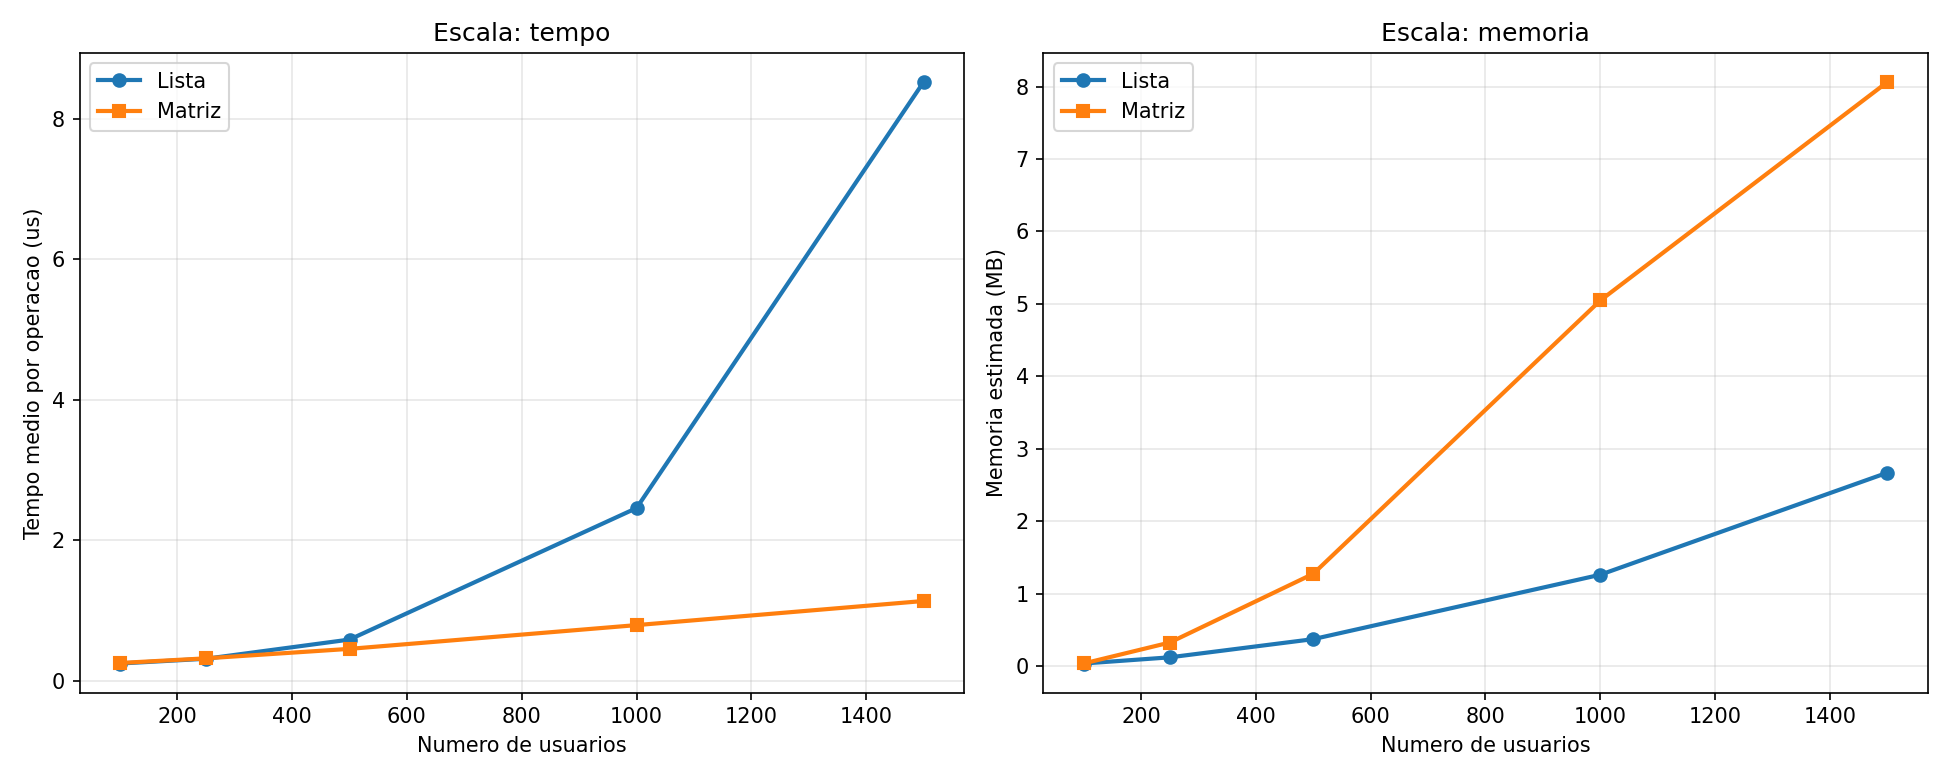
\includegraphics[width=0.75\textwidth]{../analysis/figura_1_escala_memoria.png}
    \caption{Impacto do número de usuários no tempo médio e na memória estimada.}
    \label{fig:escala-memoria}
\end{figure}

Para redes pequenas, as duas representações têm tempos próximos. Porém, a partir de
1000 usuários, a lista passa a crescer mais rapidamente. Com 1500 usuários, a lista teve
tempo médio de aproximadamente $14{,}2\mu s$ por operação, enquanto a matriz ficou em
cerca de $1{,}2\mu s$.

Em memória, ocorre o oposto: a matriz cresce mais rápido, pois depende
do quadrado do número de vértices. Para 1500 usuários, a matriz usou cerca de 8 MB,
enquanto a lista ficou em aproximadamente 2,7 MB. Esse é o principal tradeoff do
experimento: a matriz consulta arestas mais rápido, mas paga por isso em memória.

\subsection{Impacto da densidade}

A Figura~\ref{fig:densidade-memoria} mostra o efeito da densidade do grafo social. Nesse
experimento, o número de usuários e temas foi mantido fixo, variando apenas a densidade
social de 0,005 até 0,20.

\begin{figure}[H]
    \centering
    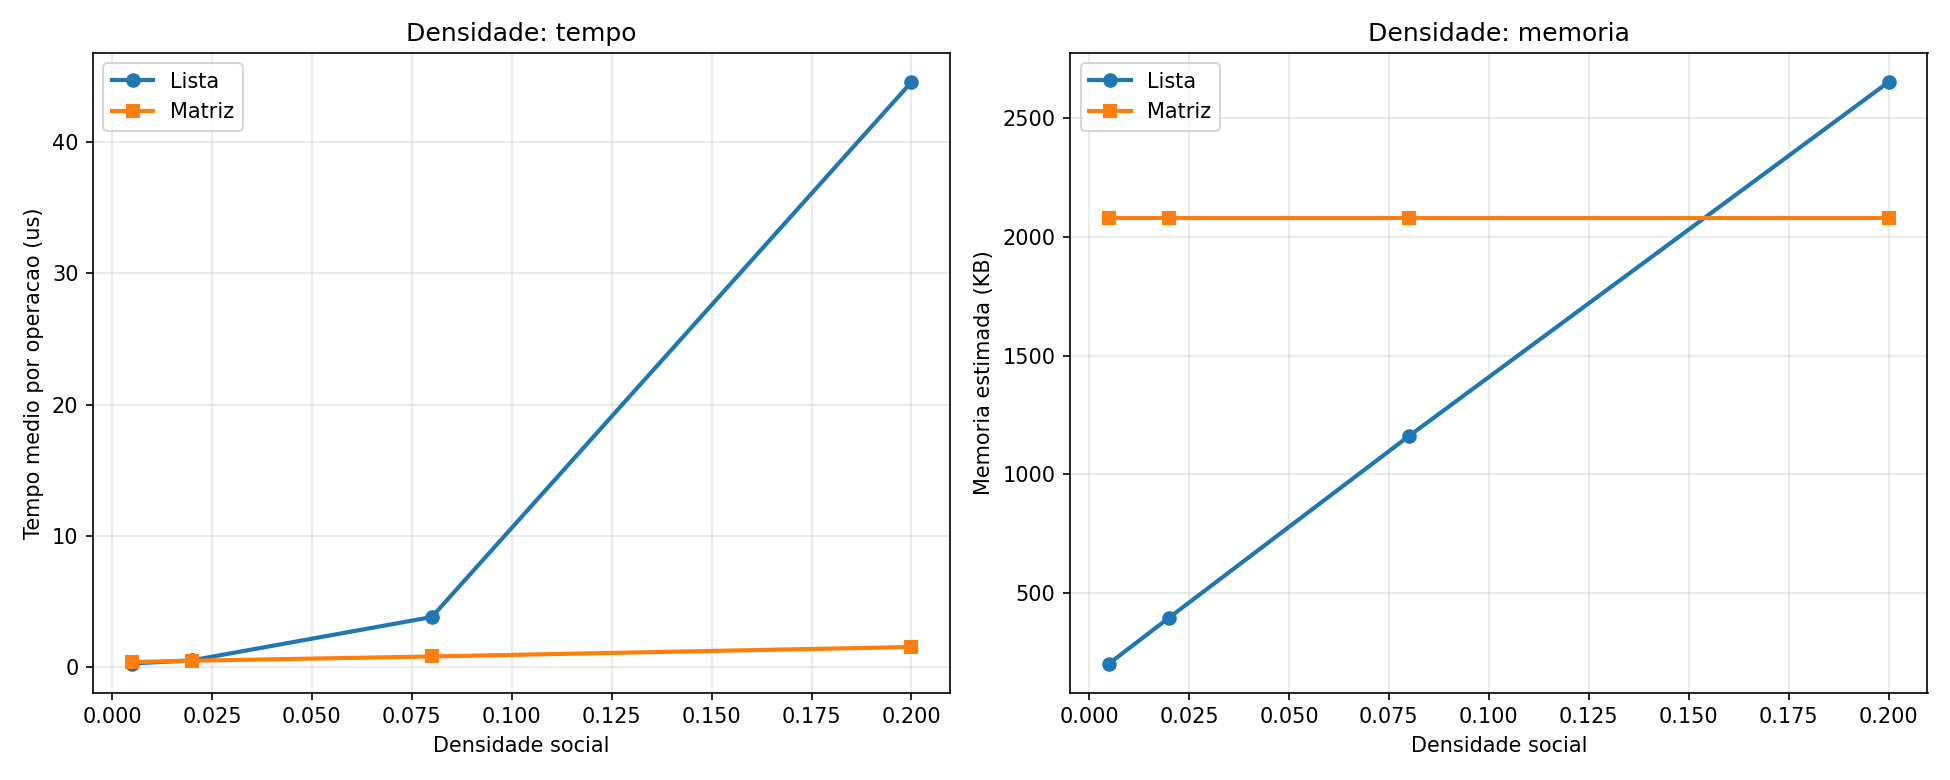
\includegraphics[width=0.75\textwidth]{../analysis/figura_2_densidade_memoria.png}
    \caption{Impacto da densidade do grafo social no tempo médio e na memória estimada.}
    \label{fig:densidade-memoria}
\end{figure}

Com densidade baixa, a lista é competitiva, pois as listas encadeadas são pequenas.
Com a densidade em 0{,}005, a lista ficou um pouco mais rápida que a matriz. Porém, conforme a
densidade aumenta, o custo de percorrer listas maiores passa a pesar bastante. Em
0{,}20 a lista chegou a cerca de $87{,}3\mu s$ por operação, enquanto a matriz
ficou em torno de $1{,}7\mu s$.

A memória também reflete esse comportamento. A matriz permanece praticamente constante,
pois seu tamanho depende apenas do número de vértices. Já a lista cresce com o número
de arestas. No cenário mais denso, a lista passou a usar mais memória que a matriz, porque
o custo das células se tornou maior que o custo da matriz.

\subsection{Impacto dos temas}

A Figura~\ref{fig:temas} avalia o grafo de temas. Foram feitos dois experimentos: no
primeiro, variou-se o número total de temas mantendo fixa a quantidade de temas por
usuário; no segundo, manteve-se fixo o número total de temas e variou-se a quantidade de
temas associados a cada usuário.

\begin{figure}[H]
    \centering
    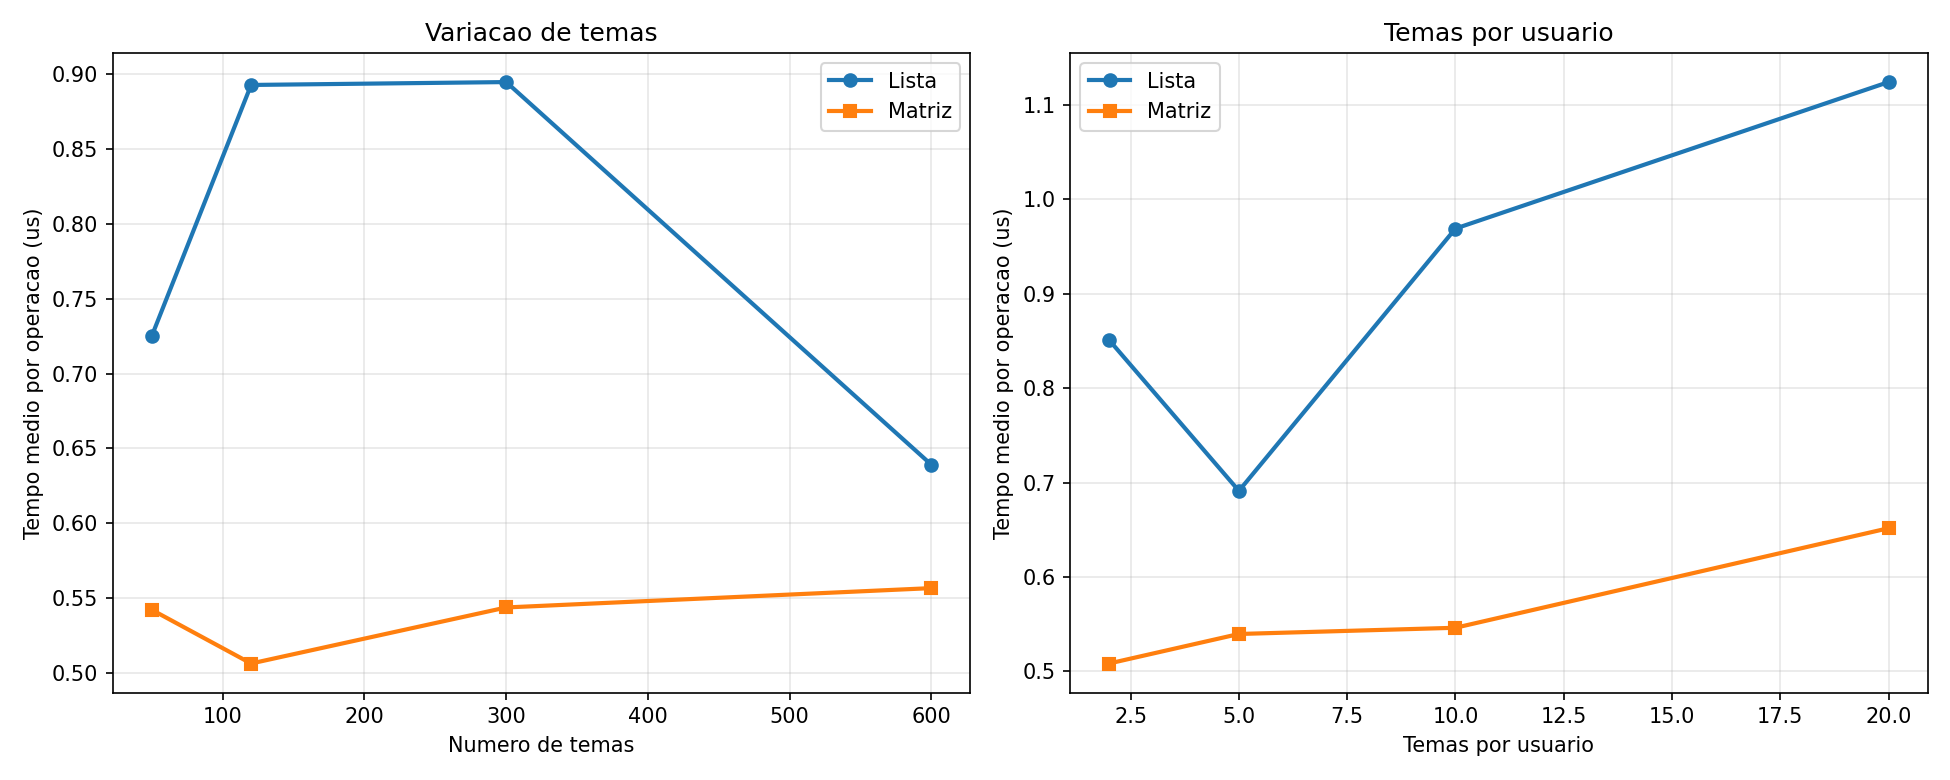
\includegraphics[width=0.75\textwidth]{../analysis/figura_3_temas.png}
    \caption{Impacto do número de temas e da quantidade de temas por usuário.}
    \label{fig:temas}
\end{figure}

A variação do número total de temas teve impacto pequeno no tempo médio nos cenários
testados, pois a carga medida mistura operações sociais e operações sobre temas. Mesmo
assim, a matriz se manteve mais estável. Já a quantidade de temas por usuário teve efeito
mais claro: quando esse valor aumenta, o número de arestas no grafo de temas também
aumenta, e a lista passa a gastar mais tempo para percorrer vizinhos.

Esse comportamento combina com a implementação. Na lista, consultas como \texttt{LT} e
\texttt{F} dependem diretamente da quantidade de vizinhos. Na matriz, o custo depende
mais do número total de vértices, pois é necessário varrer linhas ou colunas da matriz.

\subsection{Operações, perfis de carga e migração}

A Figura~\ref{fig:operacoes} compara operações isoladas e também o efeito de diferentes
perfis de carga e frequências de migração. Nesse gráfico, os três primeiros grupos do subgráfico da direita correspondem a perfis de carga, enquanto os quatro últimos variam a frequência do comando \texttt{A}.
\begin{figure}[H]
    \centering
    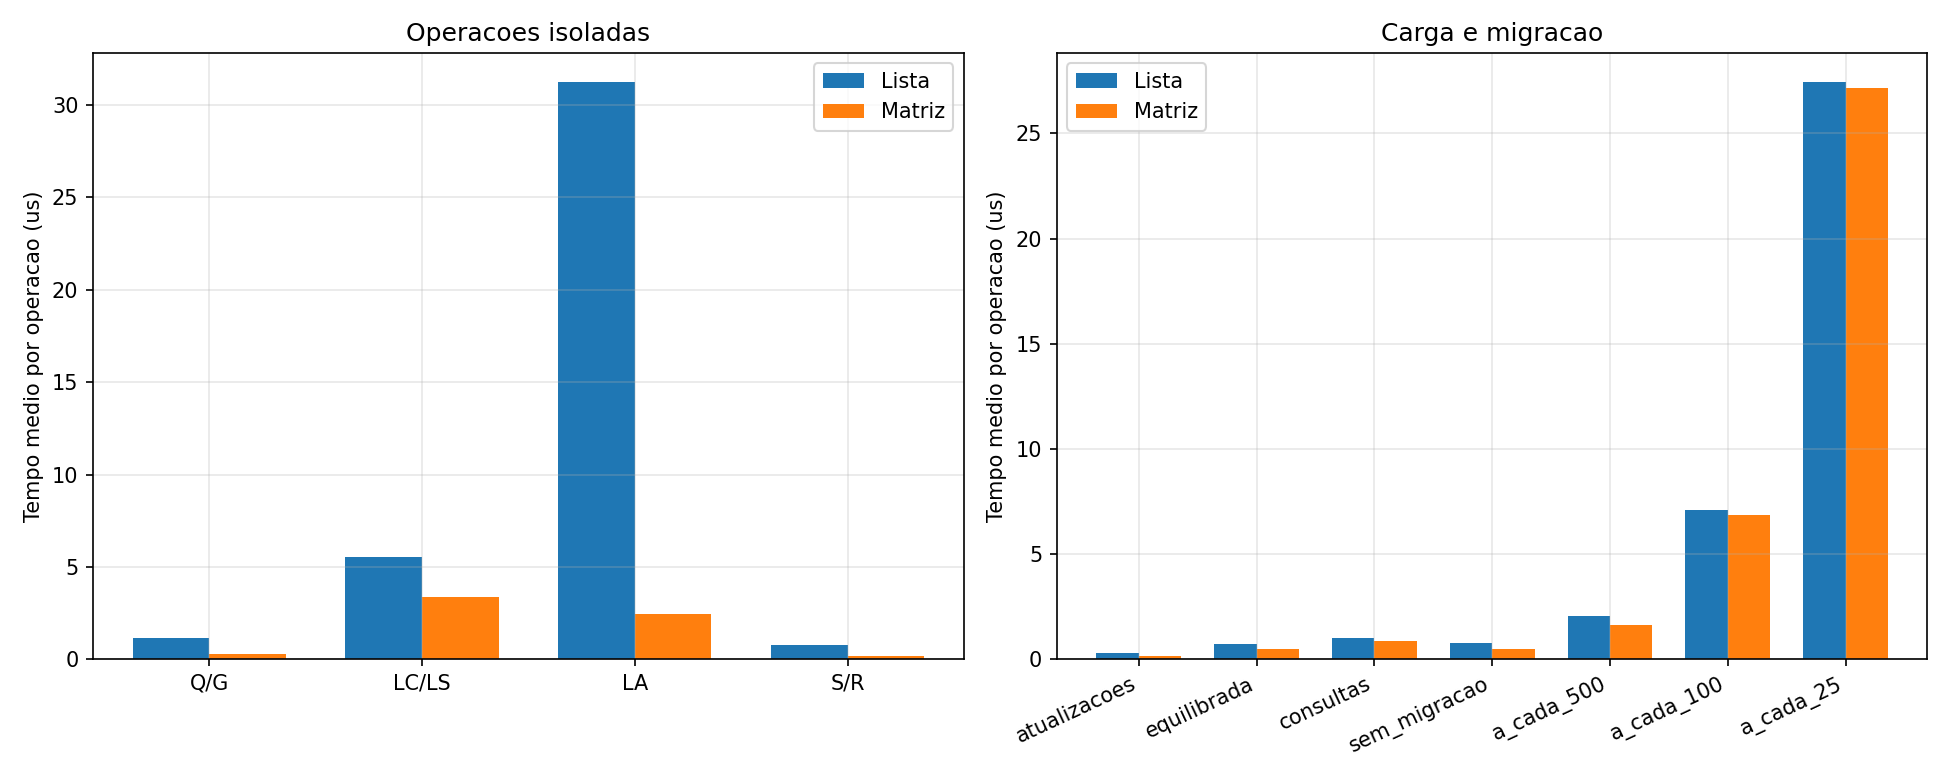
\includegraphics[width=0.75\textwidth]{../analysis/figura_4_operacoes_carga_migracao.png}
    \caption{Tempo médio por tipo de operação, perfil de carga e frequência de migração.}
    \label{fig:operacoes}
\end{figure}

Nas operações isoladas, a consulta \texttt{LA} foi a mais cara na representação por lista.
A explicação está na forma como ela trabalha: primeiro obtém os usuários seguidos e,
para cada um deles, verifica
se existe a aresta no sentido contrário. Em lista, essa verificação pode exigir percorrer uma
lista encadeada. Em matriz, o teste de aresta é direto, com acesso à posição $[i][j]$.

As consultas \texttt{Q} e \texttt{G} também favorecem a matriz, pois ambas são consultas de
existência de aresta. Já nas listagens \texttt{LC} e \texttt{LS}, a diferença foi menor, mas a
matriz ainda teve vantagem nos cenários testados, principalmente por causa da densidade
usada no experimento.

Nos perfis de carga testados, a matriz foi mais rápida nos três casos: predominância de
atualizações, carga equilibrada e predominância de consultas. A diferença aumenta nos
cenários com mais consultas, pois muitas delas dependem de verificar arestas ou percorrer
relações sociais.

A parte de migração mostra outro comportamento importante. Quando não há migração, o
custo médio permanece baixo. Porém, quando o comando \texttt{A} aparece com frequência,
o tempo cresce rapidamente. Com migração a cada 25 operações, tanto lista quanto matriz
ficaram próximas de $30\mu s$ por operação. Nesse caso, o custo dominante deixa de ser a
operação normal do grafo e passa a ser a reconstrução da representação interna.

\subsection{Conclusão da análise}

Os experimentos confirmam o tradeoff esperado entre as duas representações obrigatórias. A lista de
adjacência usa menos memória em grafos esparsos, mas seu tempo cresce bastante quando
as listas ficam longas ou quando há muitas consultas de existência de aresta. A matriz de
adjacência usa mais memória, pois seu custo depende de $V^2$, mas oferece consultas de
aresta mais rápidas e desempenho mais estável em grafos densos.

Também ficou claro que a migração entre representações pesa bastante quando aparece com frequência. Portanto,
ela deve ser usada quando há motivo para trocar o perfil de armazenamento, e não como
operação frequente. Em geral, os resultados observados acompanham a análise de
complexidade: lista tende a favorecer economia de memória em grafos esparsos, enquanto
matriz favorece consultas rápidas em redes mais densas.
\subsection{Pontos extras}
\subsubsection{Comando \texttt{P}}

A Figura~\ref{fig:comando-p} mostra o custo da consulta extra \texttt{P}, usada para
recomendar usuários. Essa consulta é mais cara que consultas simples de existência de
aresta, pois combina busca em largura no grafo social, cálculo de afinidade temática dos
candidatos válidos e ordenação das recomendações.

\begin{figure}[H]
    \centering
    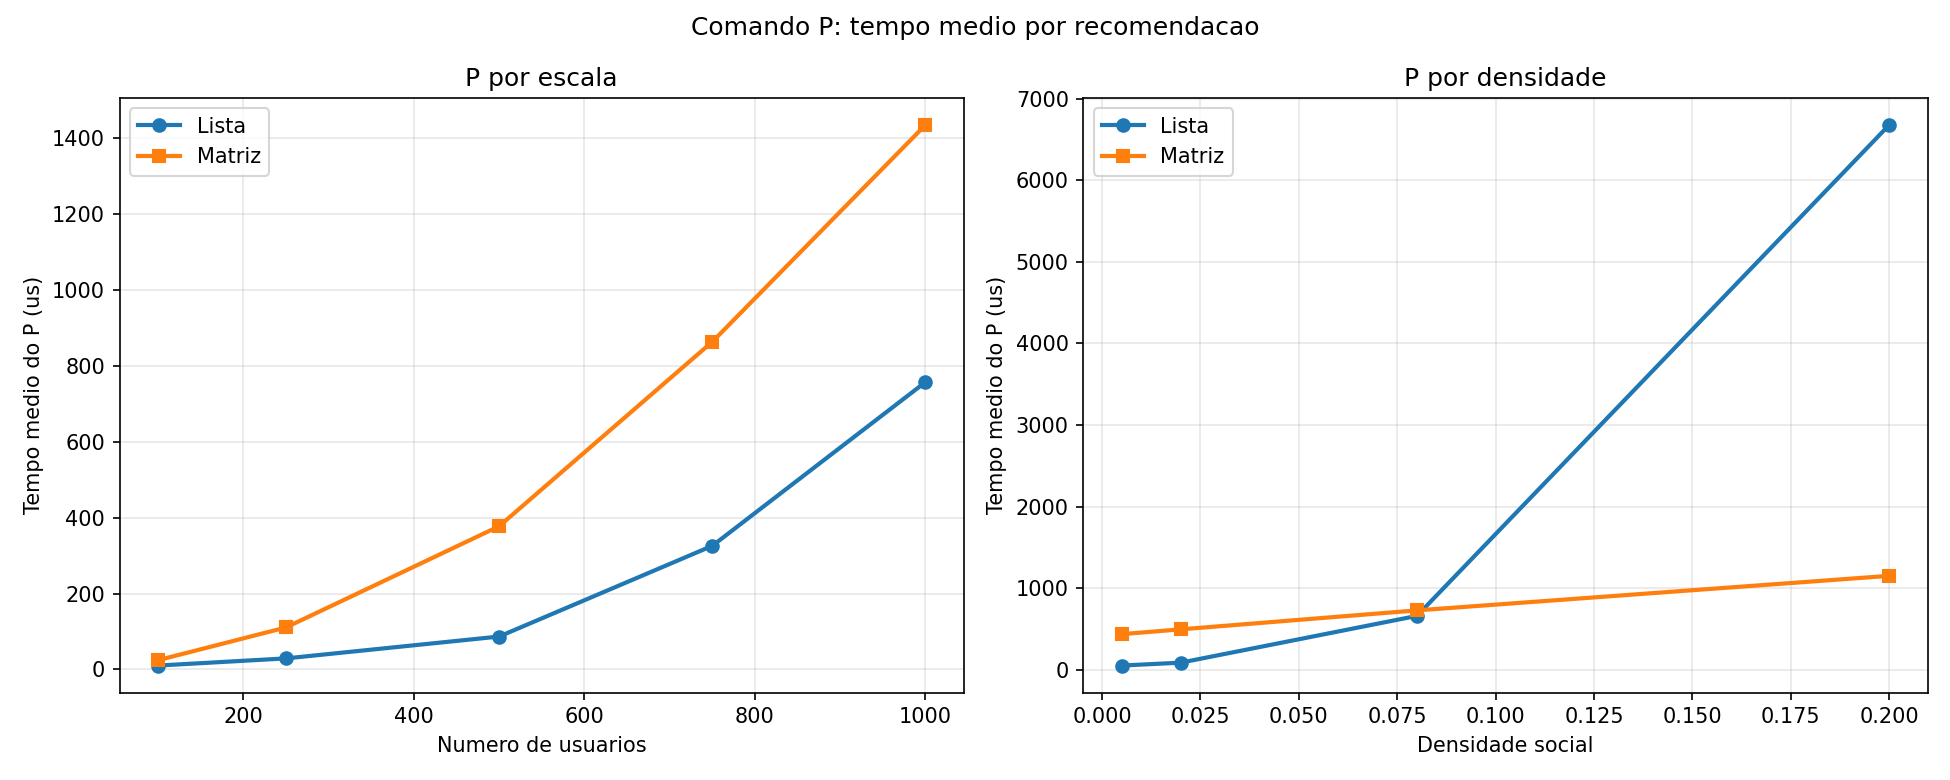
\includegraphics[width=\textwidth]{../analysis/figura_5_comando_p.png}
    \caption{Tempo médio da consulta \texttt{P} variando escala e densidade.}
    \label{fig:comando-p}
\end{figure}

No experimento de escala, as duas representações crescem com o número de usuários, mas
a lista se manteve mais rápida nos cenários testados. Com 1000 usuários, a consulta levou
aproximadamente $756{,}8\mu s$ em lista e $1434{,}1\mu s$ em matriz. Em grafos pouco
densos, a busca em largura e a coleta de temas percorrem apenas as
arestas existentes na lista, enquanto a matriz precisa varrer linhas inteiras.

No experimento de densidade, o comportamento muda nos grafos mais densos. Para
densidade baixa, a lista é melhor; porém, em densidade $0{,}20$, o tempo da lista sobe para
cerca de $6677\mu s$, enquanto a matriz fica em torno de $1152{,}6\mu s$. Nesse caso, as
listas ficam longas, e o custo de percorrê-las passa a dominar. Assim, a consulta
\texttt{P} reforça o mesmo tradeoff observado nas demais operações: lista é vantajosa em
grafos esparsos, enquanto matriz se torna mais competitiva quando a rede fica densa.

\subsubsection{Matriz esparsa}

A Figura~\ref{fig:matriz-esparsa} compara a matriz esparsa com lista e matriz nos
cenários usados para esse ponto extra. Os dois primeiros grupos variam a densidade, e os
dois últimos isolam consultas de existência de aresta e listagens.

\begin{figure}[H]
    \centering
    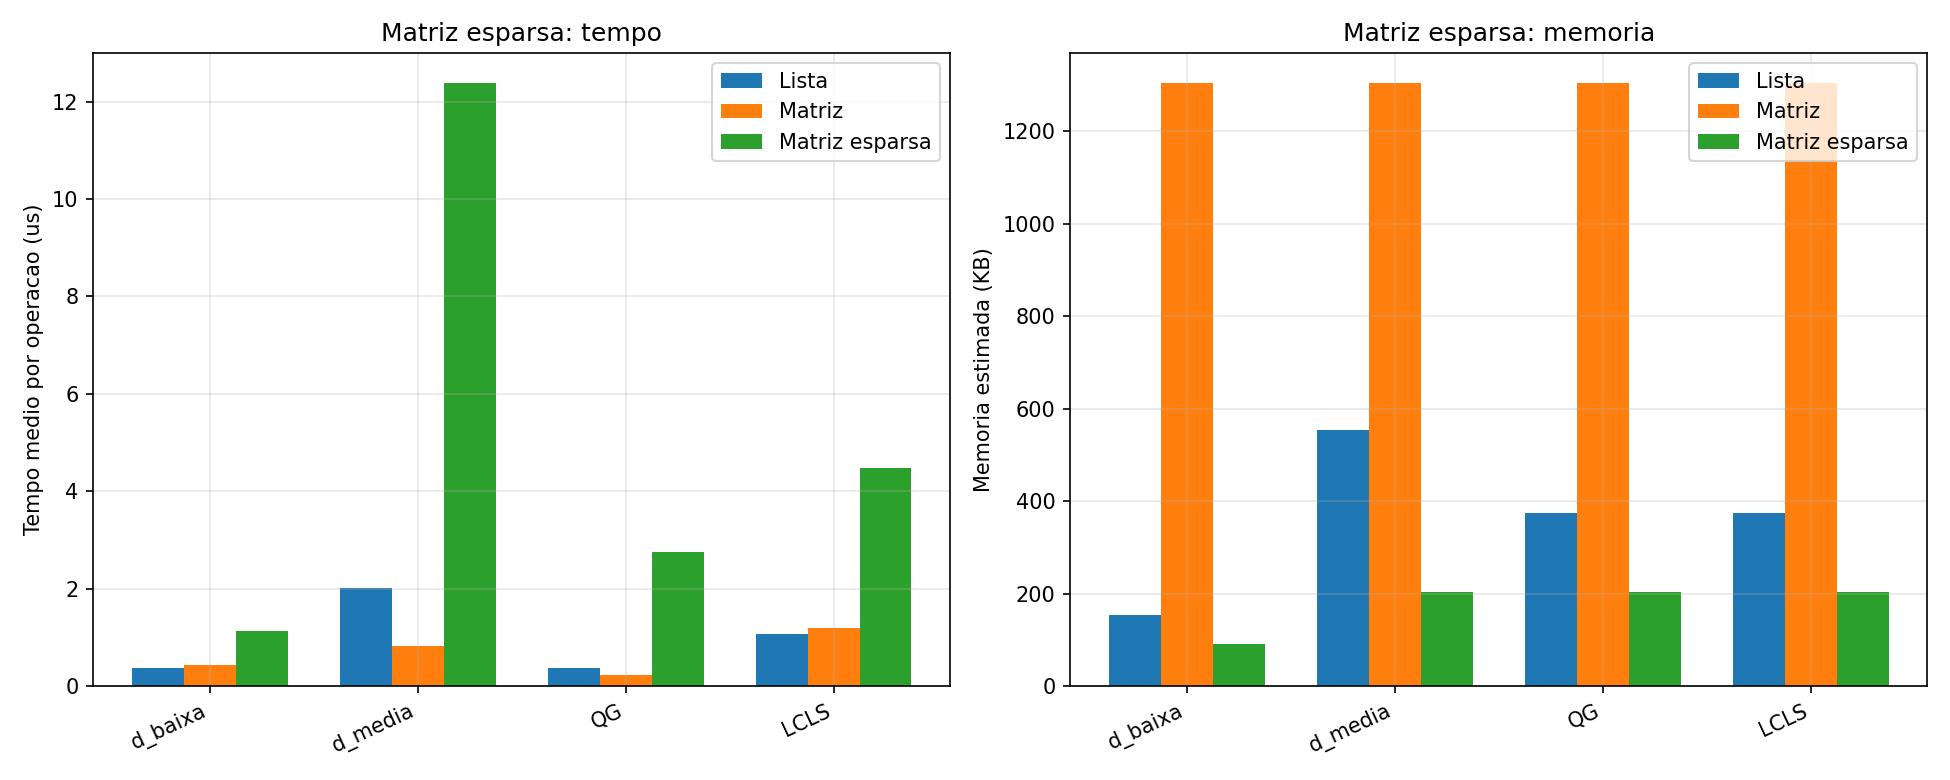
\includegraphics[width=\textwidth]{../analysis/figura_6_matriz_esparsa.png}
    \caption{Tempo médio e memória estimada usando matriz esparsa.}
    \label{fig:matriz-esparsa}
\end{figure}

O ganho de memória é o resultado mais claro. No cenário de baixa densidade, a matriz
esparsa usou cerca de 92 KB, contra 154 KB da lista e 1304 KB da matriz completa. Com
densidade média, ela ficou em aproximadamente 204 KB, ainda bem abaixo da matriz
completa e também abaixo da lista.

Em tempo, porém, a matriz esparsa não foi a melhor nos cenários testados. Como a
implementação guarda os pares em arrays simples, consultas como \texttt{Q}, \texttt{G},
\texttt{LC} e \texttt{LS} precisam percorrer esses pares para encontrar as arestas. Por isso,
ela ficou mais lenta, principalmente quando a densidade aumentou. O resultado mostra que
a representação cumpre bem o objetivo de economizar memória, mas essa economia vem com
um custo alto em tempo de busca.

\section{Conclusões}

O sistema implementado atende aos requisitos do enunciado, com as duas representações
obrigatórias do TAD Grafo funcionando corretamente e produzindo os mesmos resultados. A parte
mais trabalhosa foi manter a separação entre identificadores externos e índices internos
dos grafos, já que usuários e temas podem ter o mesmo identificador numérico. A migração
entre lista e matriz também exigiu cuidado para preservar as arestas sem duplicá-las ou
perdê-las.

Na análise experimental, ficou claro que nenhuma das duas representações obrigatórias é melhor em
todos os casos. A lista de adjacência usa menos memória em grafos esparsos, enquanto a
matriz compensa quando há muitas consultas de existência de aresta ou quando o grafo
fica mais denso. Também foi possível observar que migrações frequentes têm custo alto.
No comando \texttt{P}, o maior cuidado foi combinar busca em largura, afinidade temática
e ordenação sem misturar identificadores externos com índices internos.

A matriz esparsa, implementada como ponto extra, reforçou outro lado do problema: ela
reduz bastante o uso de memória, mas, na forma simples com arrays de pares, paga por
isso em tempo de busca.

Em suma, o principal aprendizado do projeto foi ver na prática como a escolha da
representação do grafo muda diretamente o desempenho do sistema.

\section{Bibliografia}
\begin{thebibliography}{9}
\bibitem{tp22026}
Anísio, Gisele, Wagner, Márcio (2026). \textit{Trabalho Prático 2: Modelagem de Redes Sociais Acadêmicas}. Disponibilizado via Moodle. Departamento de Ciência da Computação. Universidade Federal de Minas Gerais. Belo Horizonte.
\bibitem{edslides2026}
Anísio, Gisele, Wagner, Márcio (2026). \textit{Slides da disciplina de Estrutura de Dados}. Disponibilizado via Moodle. Departamento de Ciência da Computação. Universidade Federal de Minas Gerais. Belo Horizonte.
\bibitem{abdulbari_channel}
BARI, Abdul. \textit{Abdul Bari - YouTube Channel}. Disponível em: <\url{https://www.youtube.com/@abdul_bari}>. Acesso em: 22 abr. 2026.
\bibitem{gfg_bfs}
GeeksforGeeks. \textit{Breadth First Search or BFS for a Graph}.
Disponível em: \url{https://www.geeksforgeeks.org/dsa/breadth-first-search-or-bfs-for-a-graph/}.
Acesso em: 25 maio 2026.
\end{thebibliography}
\end{document}
